\section{Hardware Design}

Our team has one robot, called Judith (see Fig.~\ref{fig:judith}). Judith is a robot based on the Peoplebot platform~\cite{peoplebot:2001}, using a KUKA youBot arm~\cite{youbot:2016} as its main manipulator. As shown in Fig.~\ref{fig:judith}, Judith is composed of: 1 Microsoft Kinect for Xbox 360; 2 sonar arrays; 2 infrared sensors; 1 iPad 2; 1 Yoga HT-320A microphone; 1 touch sensor arrays; 2 speakers; 1 emergency button; and 1 Hokuyo URG-04LX-UG01 laser sensor.

Peoplebot has a vertical grip which was removed for the KUKA youBot arm to be attached. To attach the new arm, we built a support to keep it on the right height to manipulate objects on top of an ordinary sized table. KUKA youBot arm weighs 16.53 pounds so a wooden support was made to hang up with this weight.

\begin{figure}[ht!]
    \centering
    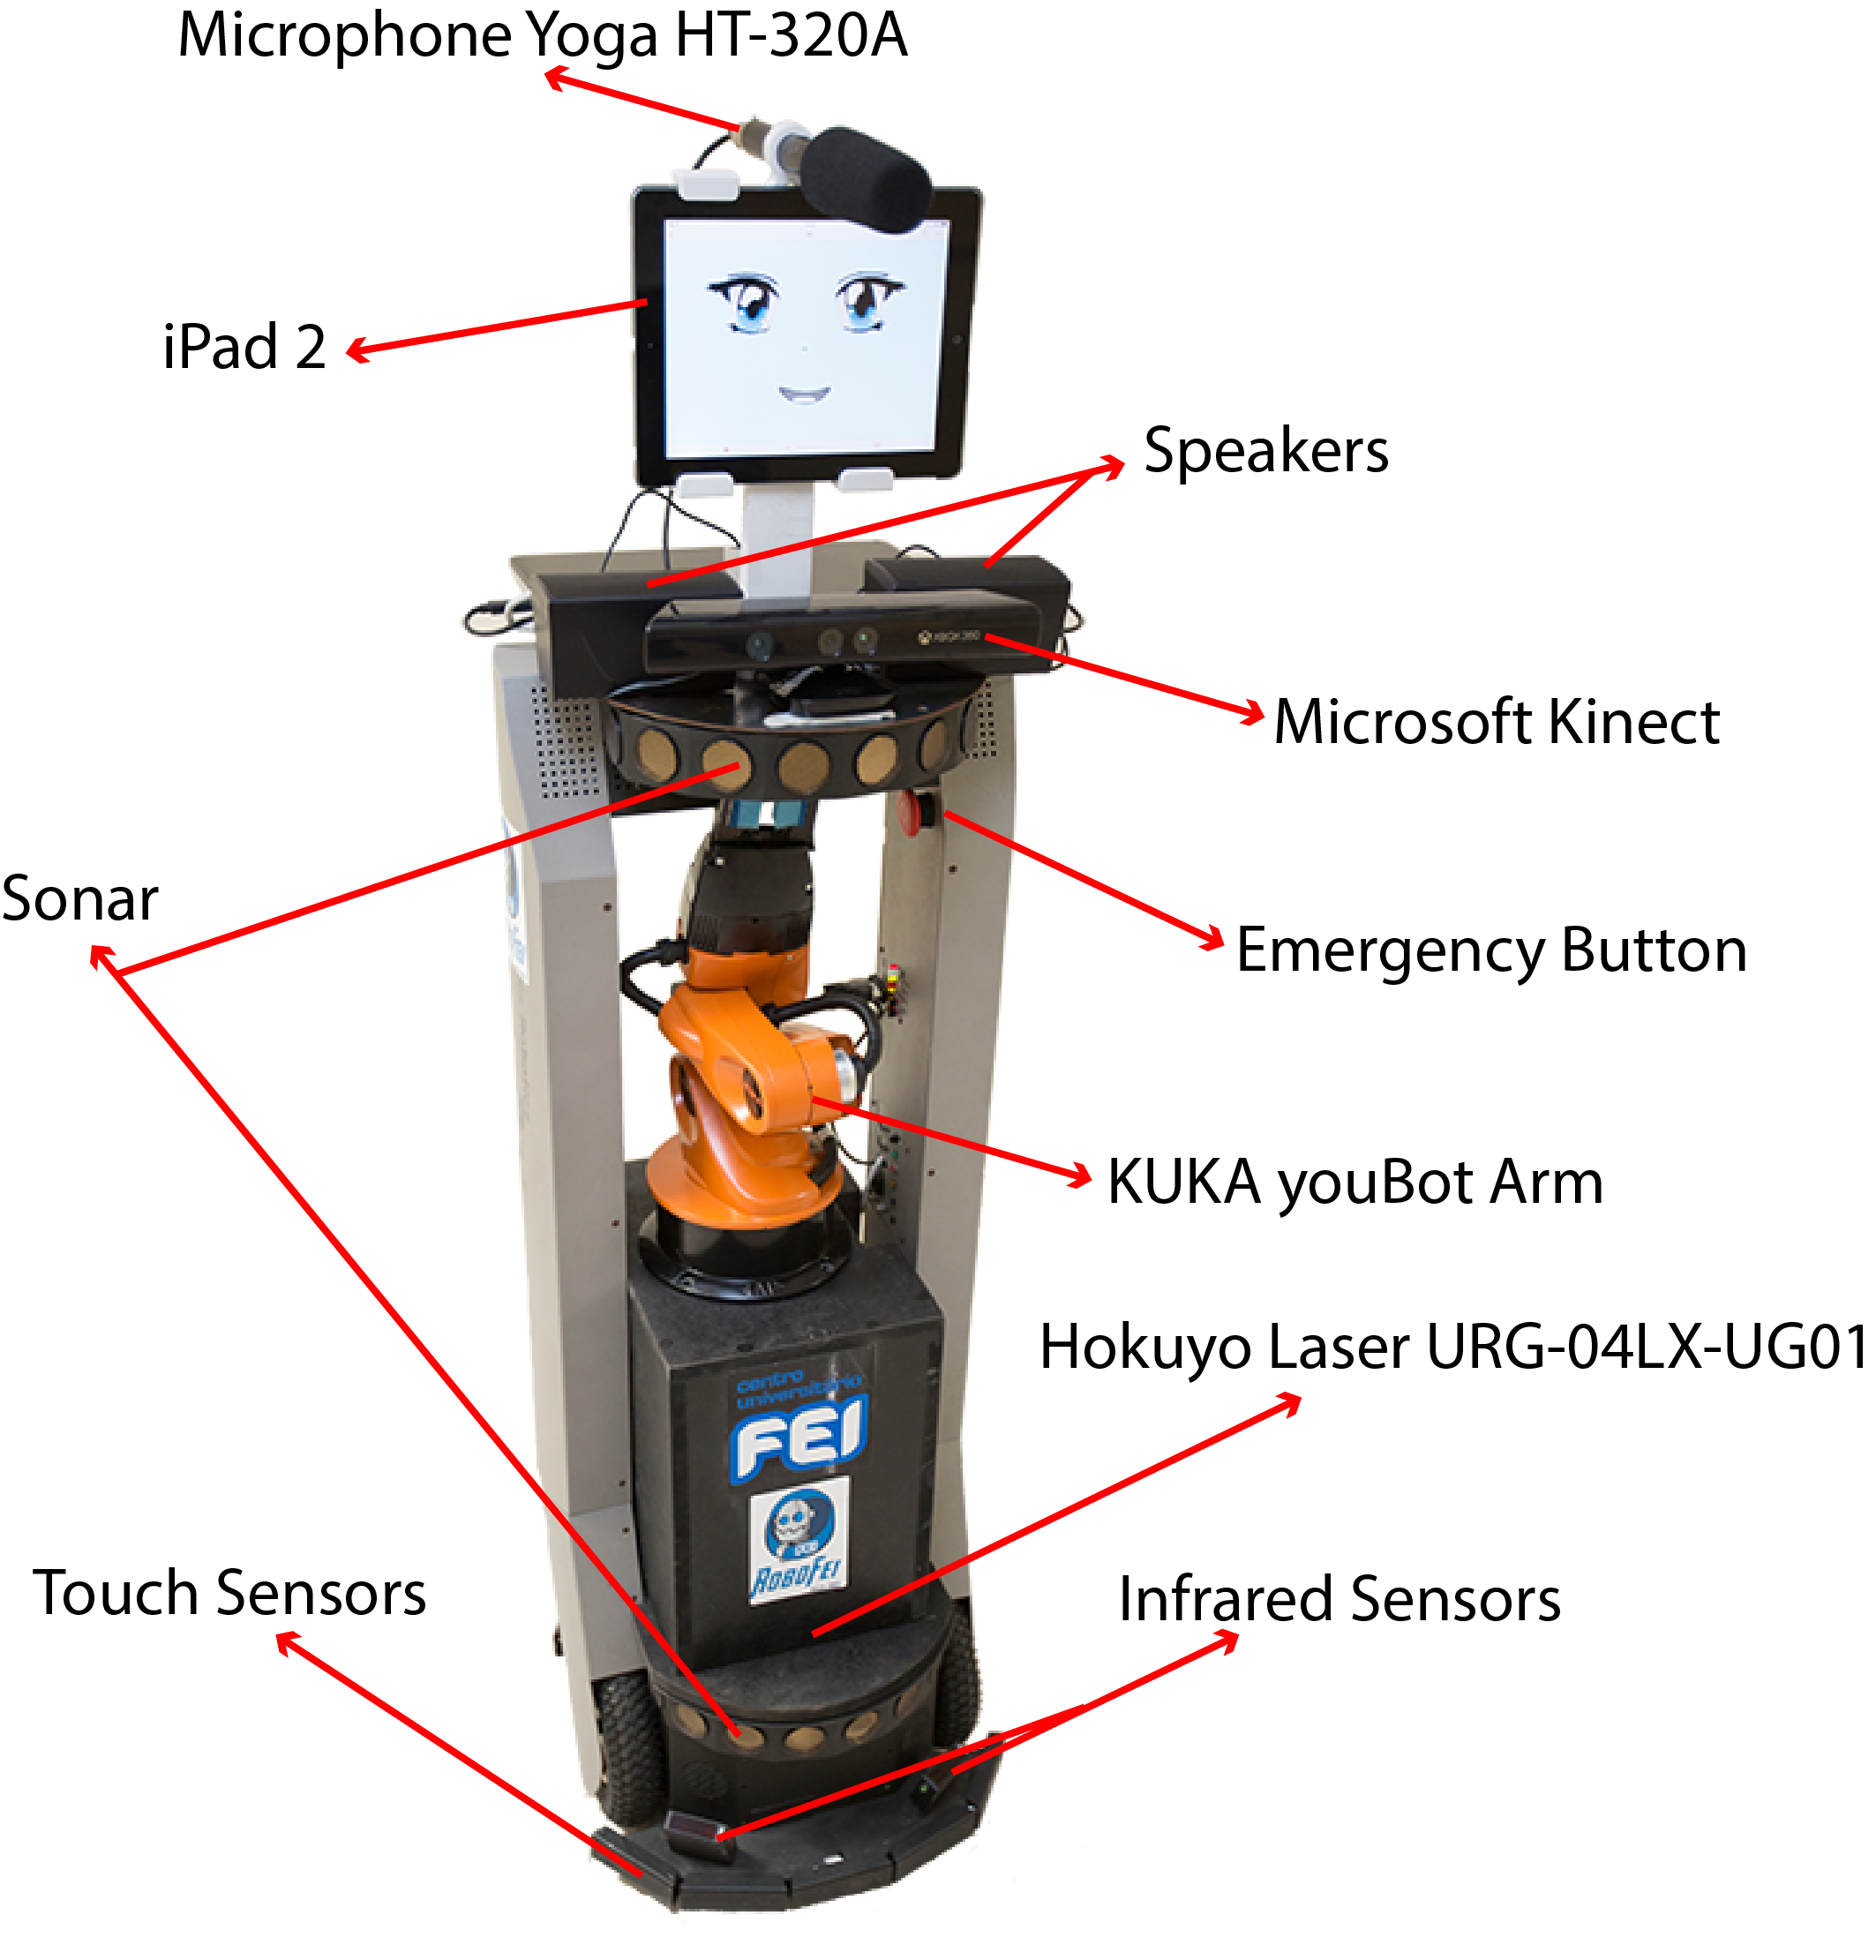
\includegraphics[height = 7.2cm]{figures/judith_info.png}
    \caption{RoboFEI's Judith}
    \label{fig:judith}
\end{figure}

Working with two different pre-manufactured robots present some challenges. First of all, each one have electric source with different voltage. KUKA youBot arm needs 24v to work while Peoplebot works with 12v. To put Peoplebot and KUKA youBot arm together, we need to build a circuit for connecting both battery kits together. This circuit is important to keep all parts of the robots safe in case of electric damage on overcharge. It also helps to make both robots work at the same time.

With both mechanical and electrical projects setups, we need to connect both robots on main computer. In order to connect Peoplebot to our laptop we used a serial RS232 to USB converter. The manipulator is able to transmit messages through an EtherCAT cable, which is connected to the computer's network port.

The robot's main computer has been an ASUS Ultrabook 14'' Touch-Screen Laptop, with an Intel Core i5, 4GB Memory, 500GB Hard Drive. It has only 3 USB ports supporting all devices, so an USB hub is used to enable more ports and increase the number of interfaced devices. As the iPad needs a paid annual license for software development, a change is being made towards Android technology so as to allow us to develop an interactive face for Judith.

The platform used by Peoplebot makes transportation a challenge, so we have worked on a modular platform using a combination of 3D print technology and aluminum parts. We want to accomplish this project until RoboCup 2016 in Germany.
